\input{../../header.tex}

\usepackage{tikz}
\usetikzlibrary{chains}
\usetikzlibrary{shapes.geometric}

\usepackage{booktabs}

\hypersetup{
    pdftitle=
}

\subject{Praktikumsprotokoll}
\title{Nukleare Elektronik und Lebensdauermessung}
\subtitle{Versuch P525 -- Universität Bonn}
\author{
    Martin Ueding \\ \small{\href{mailto:mu@martin-ueding.de}{mu@martin-ueding.de}}
    \and
    Lino Lemmer
}
\publishers{Tutor: Philipp Hoffmeister}

\begin{document}

\maketitle

\tableofcontents

\chapter{Theorie}

\section{Zerfallsschema von ${}^{22}\text{Na}$ und ${}^{133}\text{Ba}$}

Das Moseley'sche Gesetz gibt die Frequenz der charakteristischen Röntgenstrahlung eines Kerns mit Kernladung $Z$ an: \parencite[(17.10)]{meschede-gerthsen_24}
\begin{equation}
    \label{eq:moseley}
    E = h \nu = \frac 34 R_\infty c \cdot (Z - 1)^2.
\end{equation}

Nach dem Moseley'schen Gesetz \eqref{eq:moseley} ist die Energie der $K_\alpha$-Röntgenstrahlung
von Barium \SI{<< E_K_alpha_Ba_keV >>}{\kilo\electronvolt}.

\section{Wechselwirkung von $\gamma$-Strahlung mit Materie}

Trifft $\gamma$-Strahlung auf Materie, finden abhängig von Photonenergie und
Ordnungszahl des Atoms unterschiedliche Effekte statt. Die Abhängigkeit ist in
Abbildung~\ref{fig:wechselwirkung} skizziert.
\begin{figure}
    \centering
    %\includegraphics[.5\textwidth]{../Abbildungen/Wechselwirkung_Demtroeder.pdf}
    \caption{%
        Dominierende Wechselwirkung zwischen $\gamma$-Strahlung und Materie in
        Abhängigkeit von Photonenergie $E_\gamma$ und Ordnungszahl
        $Z$.%\parencite{Demtroeder_4}
    }
    \label{fig:wechselwirkung}
\end{figure}

\subsection{Photoeffekt}

\subsection{Compton-Streuung}

\subsection{Paarbildung}

Zerfällt ein Photon im Coulombfeld eines Atomkerns in ein
Elektron-Positron-Paar, spricht man von einer Paarbildung. Dies kann nur
stattfinden, wenn die Energie des Photons die Ruheenergie der beiden Teilchen
übersteigt, also $E_\gamma > 2m_\mathrm{e}c^2$. Zudem findet es bevorzugt bei
hohen Ordnungszahlen statt.

\section{Instrumente}

\subsection{Szintillator}

Zur Detektion von $\gamma$-Quanten verwendet man einen Kristall, zum Beispiel
Natriumiodid. Trifft nun ein $\gamma$ auf ein Elektron, wird es angeregt. Bei
der Abregung, die über Zwischenniveaus stattfindet, werden Photonen abgegeben,
welche von einem Photomultiplier eingefangen werden können.

\subsection{Photomultiplier (PM)}

\begin{figure}
    \centering
    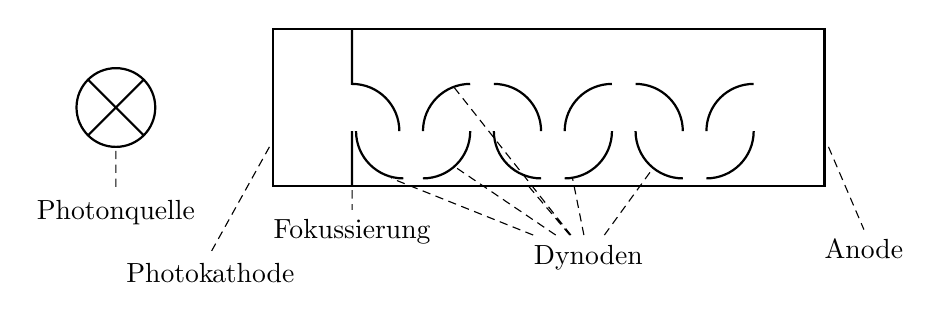
\begin{tikzpicture}
        % Röhre
        \draw[thick] (2,-1) rectangle (9,1);
        % Photonquelle
        \draw[thick]
        (0,0) circle (.5)
        (225:.5) -- (45:.5)
        (135:.5) -- (-45:.5)
        ;
        % Photokathode und Anode
        \draw[thick]
        (2,1) -- (2,-1)
        (9,1) -- (9,-1)
        ;
        % Dynoden
        \draw[thick]
        (3,-.3) -- (3,-1)
        (3,1) -- (3,.3) arc (90:0:.6cm)
        (3.05,-.3) arc (180:270:.6cm)
        (3.9,-.9) arc (270:360:.6cm)
        (3.9,-.3) arc (180:90:.6cm)
        (4.8,.3) arc (90:0:.6cm)
        (4.8,-.3) arc (180:270:.6cm)
        (5.7,-.9) arc (270:360:.6cm)
        (5.7,-.3) arc (180:90:.6cm)
        (6.6,.3) arc (90:0:.6cm)
        (6.6,-.3) arc (180:270:.6cm)
        (7.5,-.9) arc (270:360:.6cm)
        (7.5,-.3) arc (180:90:.6cm)
        ;
        % Beschriftungen PQ, PK, A und Fokussierung
        \draw[densely dashed]
        (0,-.55) -- (0,-1.05) node[below] {Photonquelle}
        (1.95,-.5) -- (1.2,-1.85) node[below] {Photokathode}
        (3,-1.05) -- (3,-1.3) node[below] {Fokussierung}
        (9.05,-.5) -- (9.5,-1.55) node[below] {Anode}
        ;
        % Beschriftung Dynoden
        \node (D) at (6,-1.9) {Dynoden};
        \draw[densely dashed]
        (D) -- (3.5,-.9)
        (D) -- (4.3,-.75)
        (D) -- (4.3,.25)
        (D) -- (5.2,-.95)
        (D) -- (5.8,-.9)
        (D) -- (6.8,-.8)
        ;
    \end{tikzpicture}
    \caption{%
        Möglicher Aufbau eines Photomultipliers
    }
    \label{fig:PM}
\end{figure}

\subsection{Splitter}

\subsection{Verstärker}

Der Verstärker/Operationsverstärker (engl. \emph{amplifier}) ist ein
elektrisches Bauteil, welches die Aufgabe hat ein eingehendes Signal zu
verstärken. Es gibt Strom-, Spannungs- und Ladungsempfindliche Verstärker, je
nach der Art des verstärkten Signales.

%TODO: Funktionsweise

\subsection{Constant Fraction Diskriminator (CFD)}

Ein Diskriminator ist ein Gerät, welches nur anspricht, wenn ein eintreffendes
Signal stärker ist, als ein bestimmter Grenzwert (engl. \emph{threshold}).
Trifft ein solches Signal ein, gibt der Diskriminator ein Standardsignal, zum
Beispiel ein Rechtecksignal aus.

Eine Anwendung des Diskriminators ist das Triggern: Trifft ein Signal ein, wird
ein neues, standardisiertes abgegeben. So ist zum Beispiel der zeitliche
Abstand zwischen zwei eintreffenden Signalen zu messen. Wann genau der
Diskriminator triggert, kommt auf die Art an.

Der CFD triggert, wenn ein bestimmter Anteil der Maximalamplitude erreicht
wird.Dazu wird das einkommende Signal gesplittet, ein Teil wird zeitlich
verzögert, der andere invertiert und um einen Faktor $k$ gedämpft. Anschließend
werden beide Signale wieder addiert. Ein vorher rein positives Signal erhält so
eine Nullstelle, welche durch $k$ bestimmt wird und den Triggerpunkt definiert.

\subsection{Einkanalanalysator (SCA)}

Der SCA ist ein elektrisches Bauteil, welches wie ein Diskriminator eine
Untergrenze hat, unter der Signale blockiert werden. Zusätzlich besitzt er eine
Obergrenze, sodass nur Signale mit einer Amplitude innerhalb eines bestimmten
Bereiches (engl. \emph{window}) betrachtet werden. Er gibt ein logisches Signal
ab, wenn die Amplitude eines einkommendes Signals aus diesem Bereich wieder
unterhalb die Untergrenze fällt.

\subsection{Vielkanalanalysator (MCA)}

Der Vielkanalanalysator sortiert einkommende Signale nach Amplitude. Trifft ein
Signal mit einer bestimmten Amplitude ein, setzt er einen Zähler in einem
bestimmten Kanal hoch. Dadurch zählt der MCA wie häufig die verschiedenen
Amplituden auftauchen. Es entsteht eine Art Histogramm.

\subsection{Koinzidenzeinheit}

Eine Koinzidenzeinheit gibt ein logisches Signal aus, wenn zwei oder mehr
eingehende Signale zeitlich überlappen. Dies kann zum Beispiel realisiert
werden, indem die Amplituden der Signale addiert werden und an einen SCA
übergeben werden, welcher so eingestellt ist, dass er nur anspricht, wenn ein
Signal mit einer Amplitude einkommt, welches der Summe aller eintreffenden
Signale entspricht.

\subsection{Zeit-Impulshöhe-Konverter (TAC)}

Wie der Name schon sagt, konvertiert ein TAC ein Zeitabstand in ein Signal mit
einer zu dieser Zeitdifferenz proportionalen Amplitude. Dies wird erreicht,
indem bei einem Startsignal ein Kondensator mit einem konstanten Strom geladen
wird. Bei einem Stopsignal wird dieser Kondensator über einen Widerstand
entladen. Die Spannung zwischen den Kondensatorplatten ist proportional zur
Zeitdifferenz und die Amplitude proportional zur Spannung. Somit ist die
Amplitude proportional zeitlichen Abstand der Eingangssignale.

\chapter{Durchführung}


Für unsere Blockschaltbilder benutzen wir folgende Notation:

\begin{tabular}{lc}
    Element & Symbol \\
    \midrule
    Analoges Signal & 
        \begin{tikzpicture} \draw[->] (0, 0) -- ++(1, 0); \end{tikzpicture}
    \\
    Digitales Signal & 
        \begin{tikzpicture} \draw[->, dashdotted] (0, 0) -- ++(1, 0); \end{tikzpicture}
    \\
    Gerät & 
        \begin{tikzpicture} \node[draw, rectangle, minimum size=1ex, draw] {}; \end{tikzpicture}
    \\
    Verstärker &
        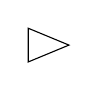
\begin{tikzpicture} \node[draw, isosceles triangle, minimum size=1ex, draw] {}; \end{tikzpicture}
\end{tabular}

\parencite{Bieling/K125}

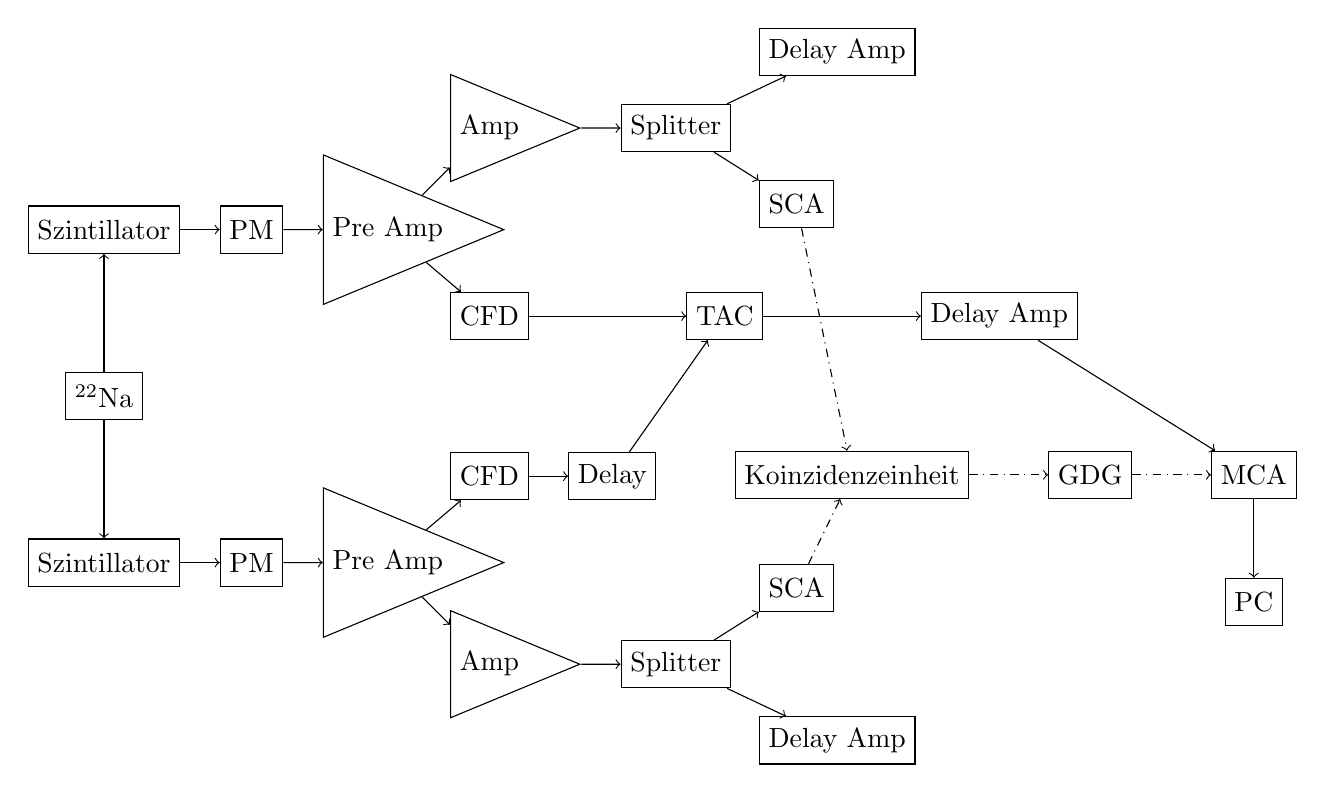
\begin{tikzpicture}[
        device/.style={
            rectangle,
            minimum size=6mm,
            draw=black
        },
        amp/.style={
            isosceles triangle,
            minimum size=6mm,
            draw=black
        },
    ]

    \node[device] (koinzidenz) at (9.5, -1) {Koinzidenzeinheit};
    \node[device] (gdg) [right=of koinzidenz] {GDG};
    \node[device] (mca) [right=of gdg] {MCA};
    \node[device] (pc) [below=of mca] {PC};

    \begin{scope}[start chain, node distance=5mm, every node/.style={join}, every join/.style={->}]
        \node[device, on chain] (22Na) at (0, 0) {$^{22}\mathrm{Na}$};

        \begin{scope}[start branch=22Na]
            \node[device, on chain=going below, node distance=1.5cm] (Szintillator1) {Szintillator};
            \node[device, on chain] (PM2) {PM};
            \node[amp, on chain] (PA2) {Pre Amp};

            \begin{scope}[start branch=PA2]
                \node[amp, on chain=going below right] (amp2) {Amp};
                \node[device, on chain] (splitter2) {Splitter};
                \begin{scope}[start branch=splitter2]
                    \node[device, on chain=going below right] (delay2) {Delay Amp};
                \end{scope}
                \begin{scope}[start branch=splitter2]
                    \node[device, on chain=going above right] (sca2) {SCA};
                \end{scope}

            \end{scope}
            \node[device, on chain=going above right] (cfd2) {CFD};
            \node[device, on chain] (cfddelay) {Delay};
        \end{scope}

        \node[device, on chain=going above, node distance=1.5cm] (Szintillator1) {Szintillator};
        \node[device, on chain] (PM1) {PM};
        \node[amp, on chain] (PA1) {Pre Amp};

        \begin{scope}[start branch=PA1]
            \node[amp, on chain=going above right] (amp1) {Amp};
            \node[device, on chain] (splitter1) {Splitter};
            \begin{scope}[start branch=splitter1]
                \node[device, on chain=going above right] (delay1) {Delay Amp};
            \end{scope}
            \begin{scope}[start branch=splitter1]
                \node[device, on chain=going below right] (sca1) {SCA};
            \end{scope}
        \end{scope}

        \node[device, on chain=going below right] (cfd1) {CFD};
        \node[device, on chain=going right, node distance=2cm, join=with cfddelay] (tac) {TAC};
        \node[device, on chain=going right, node distance=2cm] (delay3) {Delay Amp};

    \end{scope}

    \begin{scope}[->]
        \draw (delay3) -- (mca);
        \draw (mca) -- (pc);

        \begin{scope}[dashdotted]
            \draw (gdg) -- (mca);
            \draw (sca1) -- (koinzidenz);
            \draw (koinzidenz) -- (gdg);
            \draw (sca2) -- (koinzidenz);
        \end{scope}
    \end{scope}
\end{tikzpicture}

\parencite{Leo/Techniques_Nuclear_Experiments}

\hline

Wir schauen uns das Slow Signal des rechten PM auf dem Oszi an.

Danach betrachten wir das Signal nach dem Vorverstärker (Bildzeit 14:58).

Wir schließen den Hauptverstärker nach dem Vorverstärker an. Dessen Ausgang betrachten wir auf dem Oszi. (Bildzeitpunkt 15:03)

\chapter{Auswertung}

\chapter{Ergebnis}

\IfFileExists{\bibliographyfile}{
    \printbibliography
}{}

\end{document}

% vim: spell spelllang=de
